\documentclass[9pt]{article}
\usepackage[left=1in, right=1in, bottom=1in, top=1in]{geometry}
\usepackage{amsmath, amssymb, amsthm}
\usepackage{graphicx}
\usepackage{epstopdf}
\usepackage{subfigure}

\title{PGS Suspension Solver}

\begin{document}
\maketitle

The suspension can be modeled as two rigid bodies, the bar and the wheel. The bar is connected to a socket with a prismatic constraint, and the socket moves with some specified motion $x_s(t)$. The wheel connects to the bar with positional constraint. The bar is attached to a spring at its center of mass, which acts as an external force on the bar.

\begin{center}
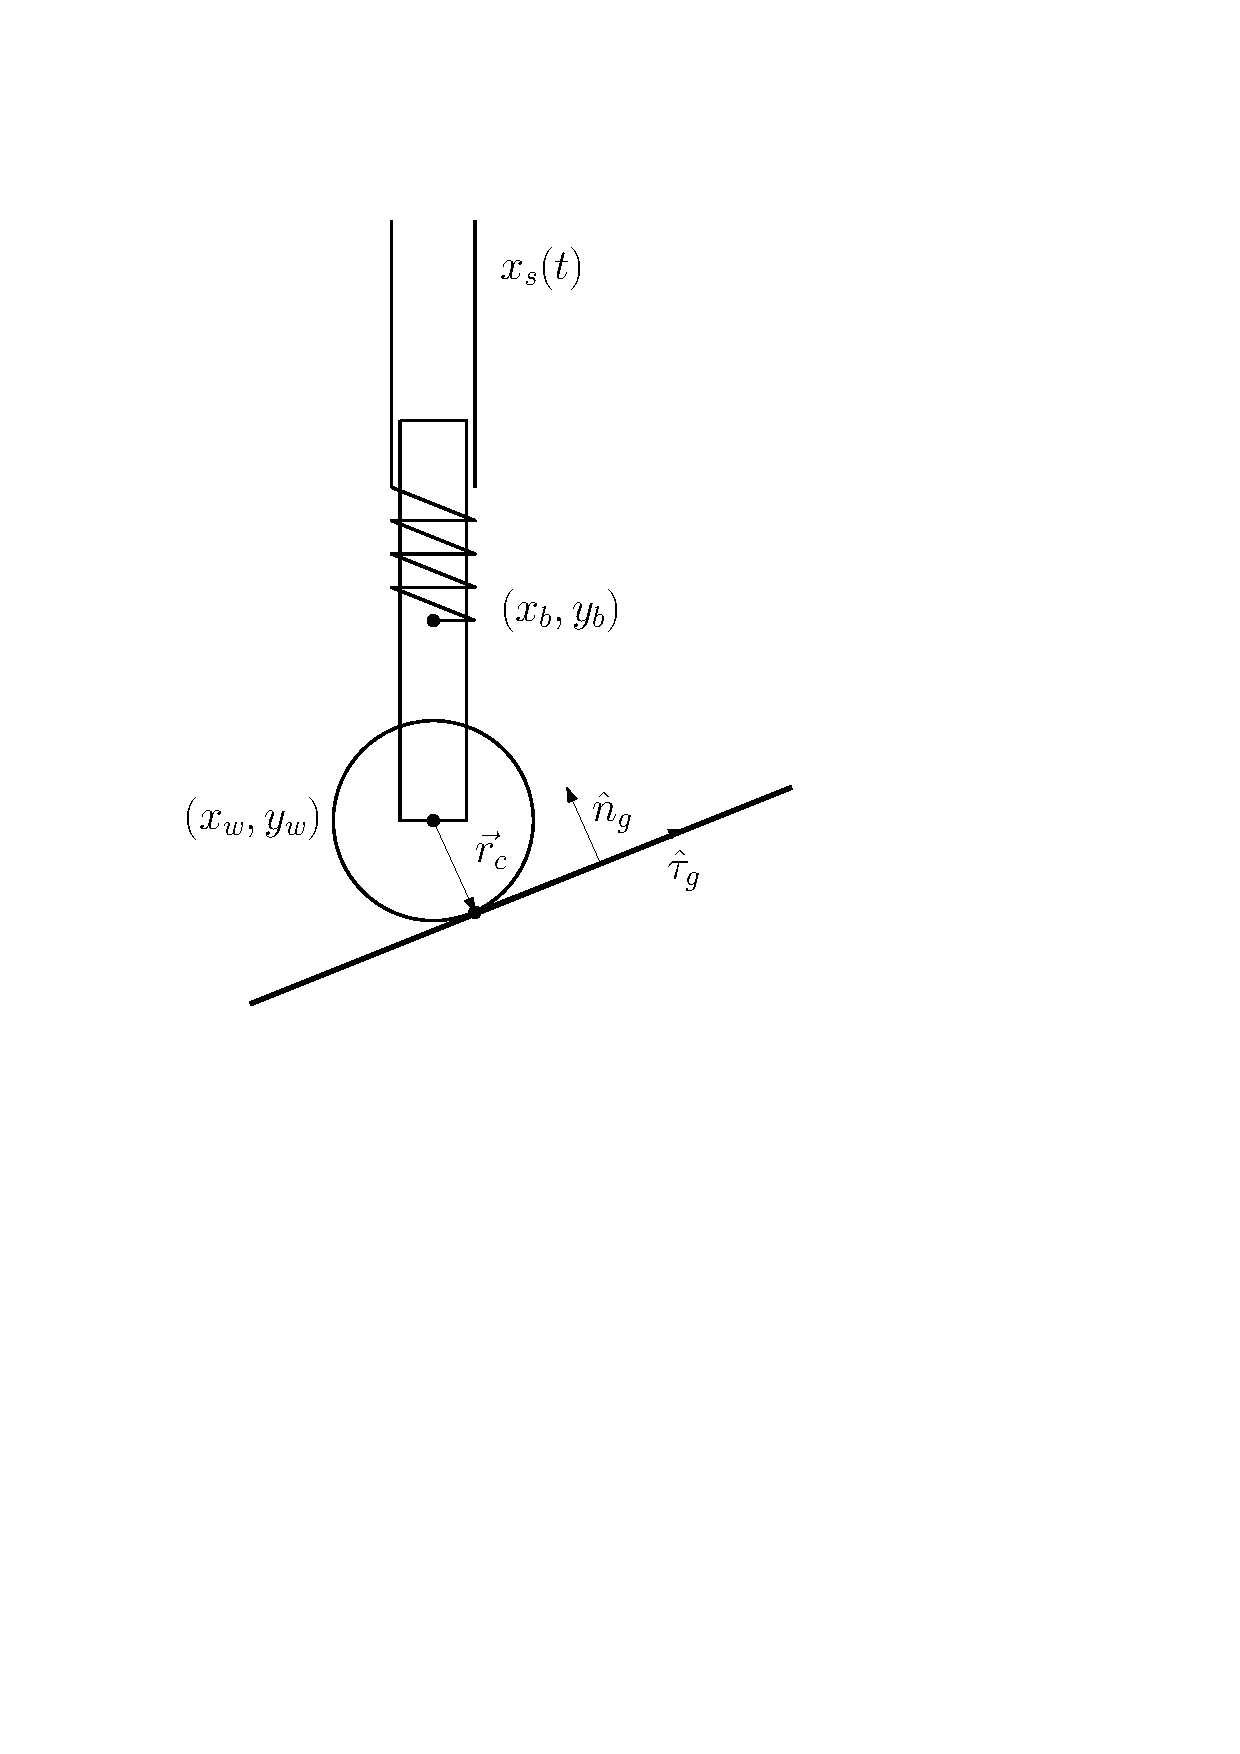
\includegraphics[scale=0.5]{diagram.pdf}
\end{center}

Each constraint introduces linear and angular impulses:
\[
\overrightarrow{\lambda}_i = 
\left[
\begin{array}{c}
\lambda_{lin} \\
\lambda_{rot}
\end{array} 
\right]
\]
The location of these impulses depends on the constraint, and will change the form of the Jacobian.

The first constraint we consider is the prismatic constraint of the bar/socket system. We have that 
\[
x_b = x_s(t) \implies u_b = \dot{x}_s(t)
\]
\[
\omega_b = \omega_s 0
\]

The second constraint is the position constraint for the wheel/bar system. 
\[
x_w - \left(x_b + \frac{L}{2}\sin \theta_b\right) = 0 \implies u_w - u_b - \frac{L}{2}\cos \theta_b \omega_b = 0
\]
\[
y_w - \left(y_b - \frac{L}{2}\cos \theta_b\right) = 0 \implies v_w - v_b + \frac{L}{2}\sin \theta_b \omega_b = 0
\]

We first solve for the constraint impulses:
\[
J V_1 = J (V_0 + M^{-1} F_{ext} \Delta t) + J M^{-1} J^T \lambda
\]
and then update the velocities:
\[
V_1 = V_0 + M^{-1} F_{ext} \Delta t + M^{-1} J^T \lambda
\]
All components of $JV_1$ are zero except where we have elastic collisions or a specified motion, such as that of the bar/socket system. For this constraint, we have that 
\[
JV_1^{c0} = 
\left[
\begin{array}{c}
u_s(t + \Delta t) \\
0 \\
0
\end{array} 
\right]
\]
The inverse mass matrix is 
\[
M^{-1} = 
\left[
\begin{array}{cccccc}
\frac{1}{m_b} & 0 & 0 & 0 & 0 & 0 \\
0 & \frac{1}{m_b} & 0 & 0 & 0 & 0 \\
0 & 0 & \frac{1}{I_b} & 0 & 0 & 0 \\
0 & 0 & 0 & \frac{1}{m_w} & 0 & 0 \\
0 & 0 & 0 & 0 & \frac{1}{m_w} & 0 \\
0 & 0 & 0 & 0 & 0 & \frac{1}{I_w} \\
\end{array} 
\right]
\]
The forcing vector is 
\[
F_{ext} = 
\left[
\begin{array}{c}
f_{sp,x} \\
f_{sp,y} - m_b g \\
0 \\
0 \\
-m_w g \\
0
\end{array} 
\right]
\]
TODO collision constraint

TODO elastic collision can be handled by not setting to zero

TODO Baumgarte stabilization

\end{document}

